\begin{frame}{Experiments}
      \begin{description}[%
        labelwidth=\widthof{Comparison}
        ]
        \item[Datasets] \textit{UCR Time Series Archive} \\85 datasets \\ predetermined train/test splits 
        \item[Hyperparameters] 
            Selected via a $5$-fold cross-validation on the training set
        % I don't mention anything about Krein SVM here for simplicity
        \item[Evaluation metric] 
            Classification accuracy
        \item[Comparison partners] 
            \begin{itemize}
                \item[--] Other kernels
                \item[--] DTW-1NN
                \item[--] State-of-the-art methods
            \end{itemize}
        \end{description}
\end{frame}

\begin{frame}{Comparison with Other Kernels}
\begin{figure}[tbp]
  \centering
  {%
    \begin{tikzpicture}[baseline, scale=0.95]
      \begin{axis}[%
        axis x line*  = bottom,
        axis y line*  = left,
        %
        mark size     = 3.0pt,
        xmin          = 0,
        xmax          = 1,
        ymin          = 0,
        ymax          = 1,
        %
        ylabel        = {$\Method{}$},  % TODO
        xlabel        = {Other kernel}, % TODO
        xtick align   = outside,
        ytick align   = outside,
        %
        %
        unit vector ratio*= 1 1 1,
        %
        legend pos     = south east,
        legend style   = {
          font              = \scriptsize,
          draw              = none,
          legend cell align = left,
          fill              = none,
        },
      ]
        \addplot[Dark2-A, only marks, mark=+] table[%
          x       = custom_rbf_kernel_SVM,
          y       = krein_wasserstein_SVM,
          col sep = comma,
        ] {data/computed_accuracies_with_baselines_new.csv};

        \addplot[Dark2-B, only marks, mark=x] table[%
          x       = linear_kernel_SVM,
          y       = krein_wasserstein_SVM,
          col sep = comma,
        ] {data/computed_accuracies_with_baselines_new.csv};

        %\addplot[Dark2-C, only marks, mark=o] table[%
        %  x       = brownian_bridge_SVM,
        %  y       = wasserstein_SVM,
        %  col sep = comma,
        %] {data/computed_accuracies_with_baselines.csv};
        %\legend{RBF, Linear, Brownian bridge}
        \legend{RBF, Linear}

        \node[anchor=west, align=left, font=\small] at (0.40, 0.35) {%
            The other kernel is better\\
            in this region
        };

        \node[anchor=west, align=left, font=\small] at (0.00, 0.90) {%
            $\Method{}$ is better\\
            in this region
        };
        % Diagonal
        \addplot[black] {x};
      \end{axis}
    \end{tikzpicture}%
  }
\end{figure}
\end{frame}

\begin{frame}{Critical Difference Plot}
    The classification performances of methods sharing horizontal bars are not significantly different.
    \begin{figure}
    % TODO: need to obtain the script to generate CD plot
      \centering
      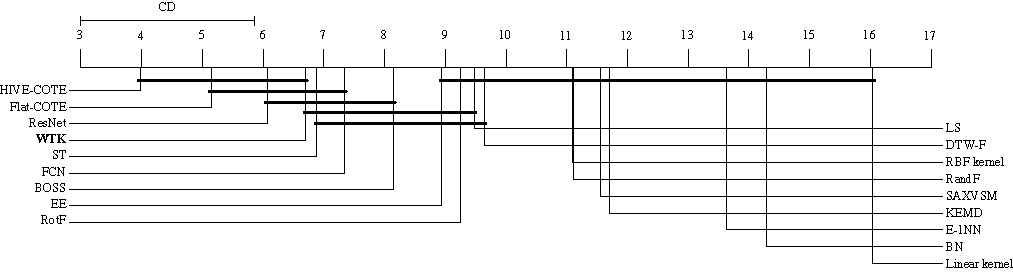
\includegraphics[width=\linewidth]{figures/CD_new.pdf}
    %   \caption{
    %     Critical difference plot, comparing our method~(shown in bold)
    %     with several other methods. The scale indicates the average rank of each method in terms of test accuracy for all data sets. The classification performances of methods sharing horizontal bars are not significantly different. We observe that there is no
    %     statistically significant difference between the performance of our
    %     method and state-of-the-art ensemble methods.
    %   }
    \end{figure}
\end{frame}